\clearpage
\section{Integrated Evidence-to-Decision Synthesis}
\label{sec:integrated_synthesis}

The contribution of this thesis is clearest when the complete evidence chain is considered rather than any single performance curve. Existing work supplies the component ideas: distributed and federated satellite systems share resources and information \citep{Golkar2015,Scrocciolani2024,Messina2025}; decentralized allocation assigns observation work across spacecraft \citep{Parjan2023,Zilberstein2025}; scheduled space networking carries data through intermittent contacts \citep{Burleigh2022,Araniti2015,CCSDS2019}; and active-fire products provide time-tagged thermal detections \citep{Wooster2005,Schroeder2014,WoosterSLSTR2012,XuWooster2023}. The step taken here is to connect those elements in one traceable experiment and ask a mission-level question: did a released task reach a suitable spacecraft before a later useful access?

That connection produces three findings that are not visible from geometric coverage alone. First, observation fulfilment and complete dissemination can move in opposite directions. The selected India event window has higher observation fulfilment than the selected California window, but lower strict dissemination completion and receiver coverage. Second, adding spacecraft improves all three percentage-based mission measures in the matched India 120-to-180 comparison, yet it also raises task traffic by about 25.8~Gbit per case. Third, increasing the Central Node fraction does not have a universal effect: bounded forwarding reverses at high fractions while the unlimited diagnostic continues to improve. The architecture question is therefore a coupled timing, routing, and resource problem rather than a coverage-maximization problem.

Figure~\ref{fig:integrated_paired_effects} places the two principal matched comparisons on one common percentage-point scale. The left panel shows why an event window cannot be described as simply ``better'' or ``worse''. The right panel shows a consistent mission benefit from the larger India fleet, but the communication-cost result must still be considered separately. The whiskers quantify stability across the enumerated base-architecture clusters; they are not probability statements about either geographic region.

\begin{figure}[htbp]
\centering
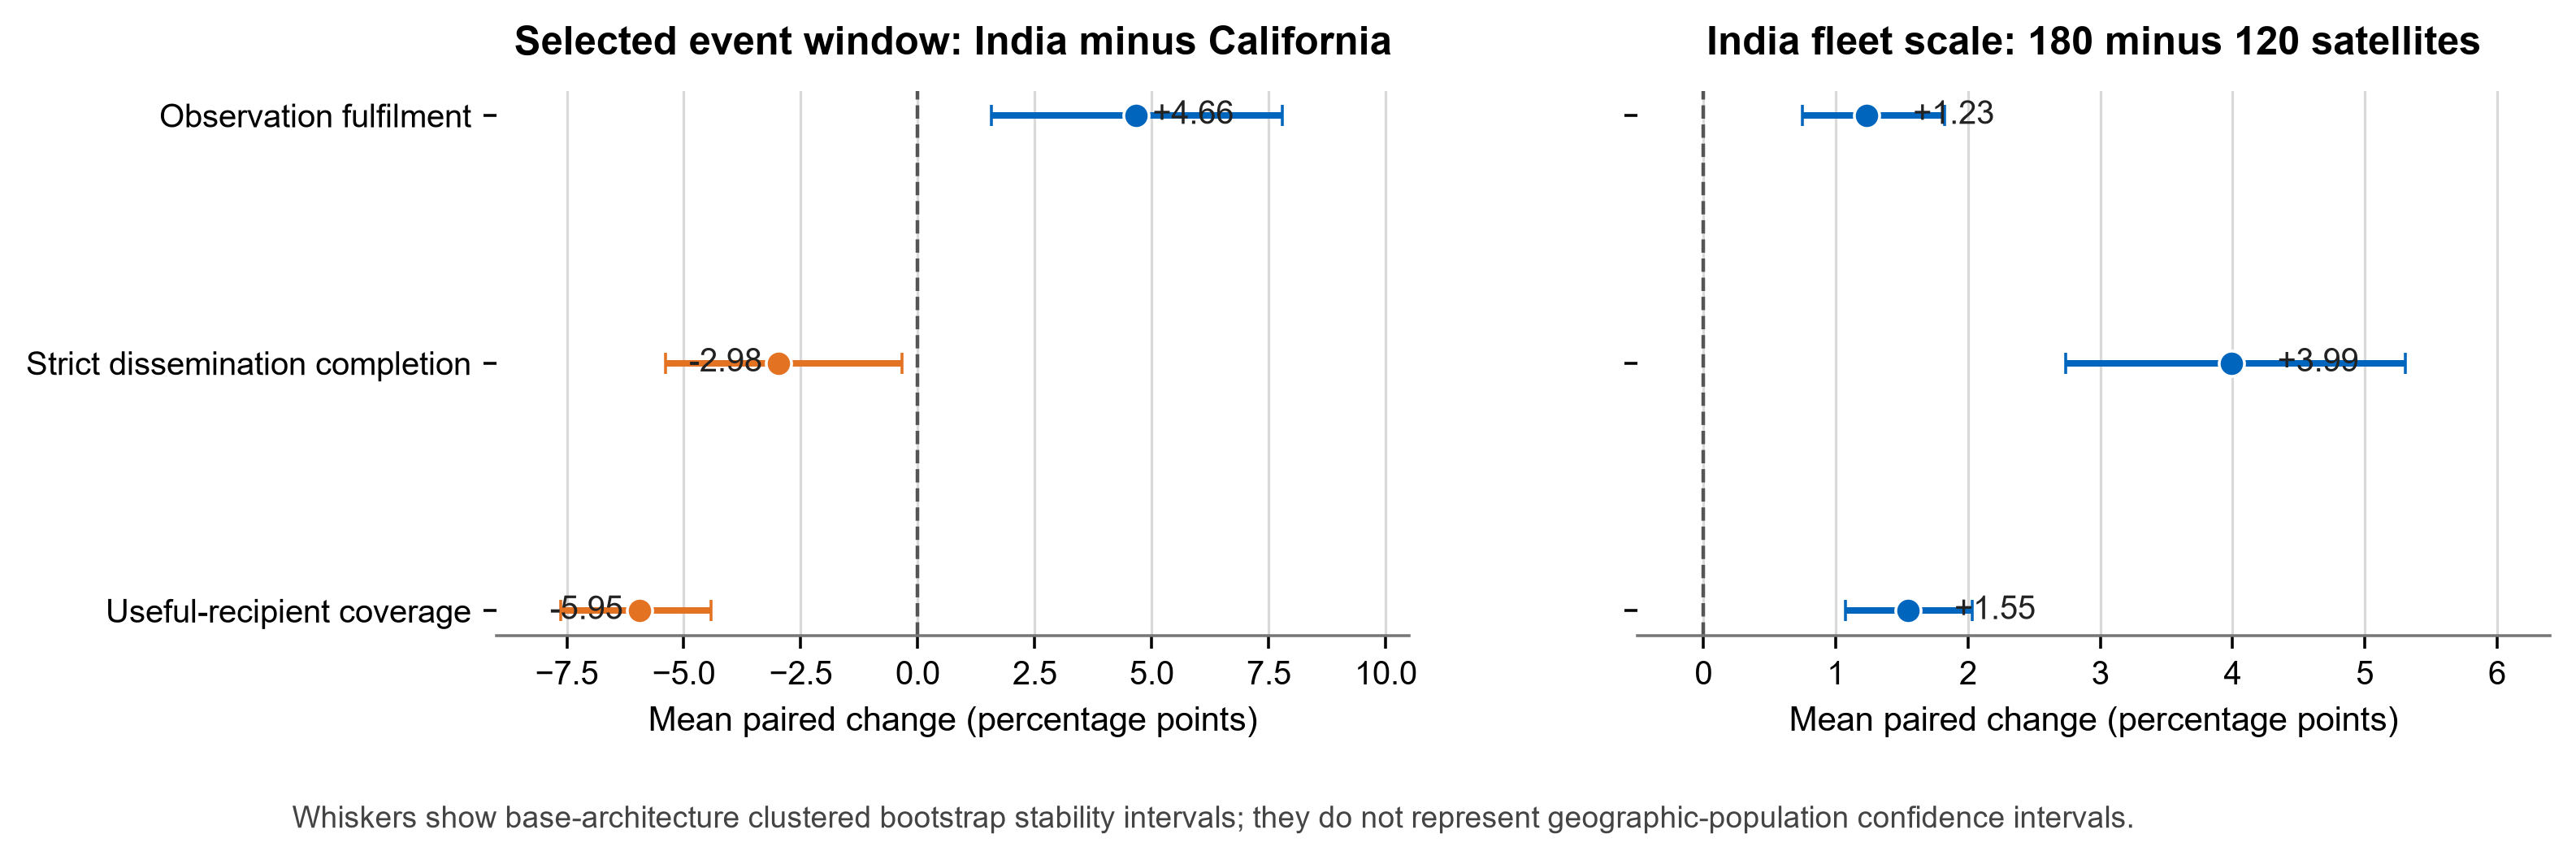
\includegraphics[width=0.98\textwidth]{figures/24_integrated_paired_effects.png}
\caption{Integrated matched effects for the three percentage-based mission metrics. The event-window panel uses 594 matched 60/120-satellite cases. The fleet-scale panel uses 216 matched India cases across 27 base architectures. Whiskers are base-architecture clustered bootstrap stability intervals.}
\label{fig:integrated_paired_effects}
\end{figure}

The resulting contribution has three layers. Methodologically, the workflow preserves release, reception, dissemination, and observation as separate events. Empirically, it identifies conditional responses to workload, routing bounds, packet size, failures, and fleet scale. For decision support, it retains non-dominated portfolios and exposes when a recommendation changes with mission preferences. This is an incremental architecture-study contribution, not a claim that Central Nodes are universally superior or that one constellation is operationally optimal.

\clearpage
\subsection{Validity and Uncertainty Budget}
\label{sec:uncertainty_budget}

The numerical results are deterministic outputs from declared simulation inputs, but the engineering interpretation still contains several forms of uncertainty. Treating all of them as sampling error would be misleading. Table~\ref{tab:uncertainty_budget} separates represented variability from assumptions that were held fixed. This distinction also explains why the report uses paired differences, base-clustered bootstrap intervals, robustness replicates, and preference sensitivity for different purposes.

\begin{table}[htbp]
\centering
\scriptsize
\caption{Uncertainty budget and its consequence for interpretation.}
\label{tab:uncertainty_budget}
\begin{tabularx}{\textwidth}{L{0.20\textwidth}L{0.22\textwidth}Y}
\toprule
Source & Representation in this thesis & Consequence for the claim \\
\midrule
Architecture variation & Enumerated Walker factors and Central Node fractions; pairing within common base identifiers & Supports comparison inside the tested grid, not inference to every possible constellation. \\
Event-window variation & Two frozen workloads with matched 60/120-satellite architectures & Establishes a workload-case contrast; it does not estimate a California or India population effect. \\
Failure realization & Thirty seeded trials for single failures and ten for combined stress & Supports mean robustness and across-trial stability; fine tail probabilities and rare-event reliability are not estimated. \\
Base-architecture heterogeneity & Clustered bootstrap over base architectures \citep{Efron1979} & Shows whether a mean effect is stable across the enumerated designs; it is not a geographic confidence interval. \\
Task construction & Fixed clustering, priority, deadline, packet-size, and \SI{700}{\kilo\metre} access rules & Results are conditional on the implemented task product and observation proxy. \\
Central Node implementation & Eligibility, preference, placement, and link-budget changes applied as one package & Package effects are identifiable, but component-specific causal effects are not. \\
Decision preference & Declared weight profiles and 10,000 reproducible family-weight draws & Measures preference sensitivity; it is not a survey of stakeholder beliefs. \\
\bottomrule
\end{tabularx}
\end{table}

The strongest internal evidence comes from comparisons that preserve the same task contract and match the same architecture identifiers. That is why the 594 regional pairs and the 216 India fleet-scale pairs carry more inferential weight than pooled marginal means. The bootstrap intervals answer a narrow question: whether the sign and approximate size of a mean paired effect remain stable when base architectures are reweighted. They do not license a null-hypothesis statement about all fires, and no such statement is required for the engineering decision made here.

Robustness trials answer a different question. Repeated failure seeds quantify sensitivity to the declared disturbance model. They do not convert an assumed failure severity into an empirical component-failure probability. Similarly, the risk matrix combines measured consequence with declared likelihood categories and must remain a screening tool, consistent with the model-validity and evidence-traceability principles used in the campaign \citep{NASA2016SEHandbook,NASAStd7009,NASA2024RiskManagement}.

The remaining uncertainty is therefore visible rather than hidden. Internal consistency is supported by task hashes, case allow-lists, recomputed metrics, matched identifiers, and frozen analysis code. External validity remains bounded by the observation proxy, two event windows, one ground station, one Central Node package, and the tested constellation levels. This division supports the numerical conclusions while preventing them from being presented as universal laws.

\clearpage
\subsection{Mechanism Interpretation and Competing Explanations}
\label{sec:mechanism_competing}

The most striking response is the high-fraction decline under bounded forwarding. The observation is secure: CN90-to-CN100 reduces observation fulfilment by about 22 percentage points in both matched event windows, and the 180-satellite bounded curve declines from 88.15\% at CN30 to 43.52\% at CN100. The mechanism is not uniquely identified because the Central Node label changes several model components together. Table~\ref{tab:mechanism_hypotheses} therefore separates explanations that are consistent with the outputs from explanations that have actually been demonstrated.

\begin{table}[htbp]
\centering
\scriptsize
\caption{Competing explanations for the high-Central-Node response.}
\label{tab:mechanism_hypotheses}
\begin{tabularx}{\textwidth}{L{0.22\textwidth}L{0.34\textwidth}Y}
\toprule
Candidate explanation & Evidence consistent with it & Evidence required to distinguish it \\
\midrule
Copy or hop limits become binding & Bounded performance reverses while the unlimited diagnostic improves toward CN100 & Per-task copy exhaustion, hop-depth, and drop-reason traces across the fraction sweep. \\
Forwarding concentration creates contention & Higher fractions change preferred paths and task traffic; large packets cause major completion losses & Queue occupancy, waiting-time, attempted-transfer, and contact-capacity utilization traces. \\
Deterministic placement changes temporal reachability & Central Nodes are distributed across planes and the selected identities change with the fraction & Randomized or optimized placements repeated under the same architecture and routing policy. \\
Link eligibility and range, rather than routing priority, drive the effect & The role changes both admissible links and a 1.5 endpoint range factor & Component ablations that vary eligibility, range, preference, and placement one at a time. \\
Workload composition changes which paths matter & Regional rank agreement is low for strict completion and packet sensitivity is large & Additional event windows with the same task-generation contract and controlled priority mixtures. \\
\bottomrule
\end{tabularx}
\end{table}

The bounded-versus-unlimited comparison is still diagnostically valuable. It falsifies a simpler explanation that high Central Node participation is intrinsically harmful under every forwarding rule. When the limits are relaxed, high fractions improve completion and timing. The decline therefore belongs to an interaction between the package and the bounded policy. It cannot be attributed to orbital geometry alone, because the same base architectures display a different response when the forwarding rule changes.

The packet-size result provides a second mechanism clue. Fourfold packets reduce strict completion by 37.02 points in the matched India block and 33.67 points in the 180-satellite extension. Larger packets consume more of each finite contact and make the same temporal route harder to complete before a deadline. This establishes capacity sensitivity at the package level. It does not prove whether queueing, contact fragmentation, or copy allocation is the dominant internal cause.

Accordingly, the thesis makes a mechanism-bounded claim: routing limits, message size, and the implemented Central Node package interact strongly enough to alter architecture ranking. Detailed trace instrumentation and component ablation are the next tests. This wording preserves the engineering meaning of the observed reversal without turning a plausible explanation into an unmeasured causal result.

\clearpage
\subsection{Operational Architecture Decision Path}
\label{sec:operational_decision_path}

The simulation does not select one flight design automatically. It narrows the decision to a portfolio and identifies which additional information would change the choice. Table~\ref{tab:decision_path} translates the evidence into architecture gates for a mission design review.

\begin{table}[htbp]
\centering
\scriptsize
\caption{Evidence-to-decision path for applying the thesis results.}
\label{tab:decision_path}
\begin{tabularx}{\textwidth}{L{0.18\textwidth}L{0.28\textwidth}L{0.23\textwidth}Y}
\toprule
Decision gate & Evidence from this thesis & Defensible provisional choice & Information required before commitment \\
\midrule
Task-message product & Packet size is among the strongest sensitivity drivers & Keep the request compact and transmit only information needed for scheduling & Confirm operational fields, encoding, authentication, and update frequency. \\
Forwarding policy & Peer/hybrid improves completion but adds substantial traffic; bounded high-CN response reverses & Use bounded routing only with explicit copy/hop verification; retain a peer-capable fallback & Trace queues, drops, contact utilization, and recovery behaviour. \\
Central Node tier & CN40/CN50 offers a lower-resource balance; CN90/CN100 can improve unlimited completion and timing & Carry both a moderate and high-participation candidate into the next trade & Separate range, placement, eligibility, and priority by component ablation. \\
Fleet scale & India 180 improves mission metrics and P100 $T_{100}$, but adds about 25.8~Gbit per case & Select 180 only if the completion and timing gains justify spacecraft and network burden & Add cost, energy, storage, launch, operations, and downlink constraints. \\
Ground segment & Ground-station outage is the strongest single failure family tested & Treat the one-station baseline as a design risk & Compare additional station locations, availability assumptions, and service cost. \\
Decision weights & Exact Pareto and rank acceptability show multiple defensible winners & Preserve the non-dominated portfolio rather than fixing an analyst-selected winner & Elicit thresholds and weights from mission operators and programme stakeholders. \\
\bottomrule
\end{tabularx}
\end{table}

The first decision is therefore not ``how many Central Nodes are best?'' but ``what operational task must be delivered, by when, and at what communication cost?'' Once that contract is fixed, infeasible architectures can be removed with explicit thresholds. Exact Pareto filtering should then precede preference weighting so that a compensatory score cannot rescue a design that is worse on every retained objective. Rank acceptability is used last to show how often each remaining candidate wins under alternative, declared preferences \citep{LahdelmaSalminen2001}.

Responsibilities are also separable. The mission scientist defines the useful observation and deadline. The communications engineer validates contact capacity and forwarding behaviour. The spacecraft architect assesses the mass, power, antenna, and processing implications of the Central Node package. The ground-segment designer addresses the single-station vulnerability. The programme decision authority supplies thresholds and preferences. The thesis provides a common evidence set for those roles, but it does not substitute analyst weights for their decisions.

For the current evidence, the defensible output remains tiered. A moderate-Central-Node candidate is appropriate when traffic and differentiated-node burden are constrained. A high-participation candidate is appropriate only under a forwarding policy that avoids the bounded reversal and when faster complete dissemination justifies the added traffic. The 180-satellite tier is an India-workload scale option, not a universal replacement for the 120-satellite cases.

\clearpage
\subsection{Adversarial Stress Test and Calibrated Claim Set}
\label{sec:adversarial_claims}

The strongest counter-argument is that the apparent architectural lessons could be artifacts of one simulator, one bundled Central Node implementation, one observation-radius proxy, one ground station, and two selected event windows. Under that interpretation, the high-fraction reversal might disappear with different placement or copy rules; the regional contrast might reflect the chosen days rather than geography; and the portfolio weights might encode analyst preference rather than mission value. This counter-argument is valid against any universal claim of superiority.

It does not invalidate the narrower thesis claim. The workflow demonstrates that reception timing must be combined with later access before a follow-up can be credited. The factorial and matched comparisons then show that, within the verified experiment, routing bounds, task size, event workload, fleet scale, and failure family materially alter the result and often alter the ranking. Those are conditional findings, and their usefulness is precisely that they reveal which assumptions must be tested before a design is frozen.

Table~\ref{tab:calibrated_claims} converts this adversarial review into a claim ledger that separates supported, suggestive, and unsupported statements and identifies what evidence could overturn each conclusion.

\begin{table}[htbp]
\centering
\scriptsize
\caption{Calibrated claim set after adversarial review.}
\label{tab:calibrated_claims}
\begin{tabularx}{\textwidth}{L{0.20\textwidth}L{0.34\textwidth}Y}
\toprule
Claim status & Claim supported by the present evidence & Boundary or falsifying extension \\
\midrule
Supported & Geometric opportunity alone overstates useful follow-up when task reception occurs too late. & A verified replay in which reception timing never changes fulfilment would contradict this result. \\
Supported & The implemented Central Node package interacts with forwarding bounds and can reverse at high fractions. & The package claim would fail if the reported bounded/unlimited outputs or matched identifiers could not be reproduced. \\
Supported & Packet size and ground-station outage are decision-relevant sensitivities in the tested campaign. & Their importance may change under a different message product or multi-station network. \\
Supported & No tested architecture dominates every mission, timing, traffic, burden, and robustness objective. & A new candidate that dominates the retained portfolio would replace the present decision set. \\
Suggestive, not causal & Copy exhaustion, routing concentration, or queue contention may explain the bounded high-CN decline. & Requires trace-level diagnostics and one-factor component ablations. \\
Not supported & Central Nodes are universally superior, one region is inherently easier, or 180 satellites are always preferable. & These statements exceed the tested workloads, package, and objective set. \\
\bottomrule
\end{tabularx}
\end{table}

The five-perspective cross-check leads to a bounded positive judgement. The research question, method, result, and conclusion form a traceable chain; the task-population correction and integrity gates address the most serious reproducibility risk; the main numerical comparisons are paired and uncertainty-qualified; and the architecture recommendation is conditional rather than absolute. No unresolved contradiction was found between the reported tables, figures, and conclusions. The remaining limitations concern transfer to new event windows, component-level mechanism attribution, and operational implementation. They require follow-on experiments, but they do not negate the thesis contribution within its declared scope.

The central result can therefore be stated without overclaiming: a preferred-relay architecture can improve time-critical task dissemination, but its value depends on forwarding limits, workload, fleet scale, communication burden, and failure tolerance. A mission-ready choice requires these quantities to be evaluated together and traced back to the task contract that produced them.
